\section{System Architecture and Virtualization}
\label{sec:architecture}

The Virtual Private Phone (VPP) reconciles the conflicting demands of comprehensive mobile utility and anti-forensic security by physically isolating storage and computation from the human interface. This section details the structural components of the frontend and backend nodes and their inter-node virtualization fabric.

\subsection{Architectural Overview}
Figure~\ref{fig:vpp_detailed_architecture} illustrates the bipartite architecture of the VPP system. The architecture separates the user experience into an ephemeral, peripheral-only edge device (the Frontend Handset) and a hardened, persistent compute core (the Backend Core).

\begin{figure}[h!]
\centering
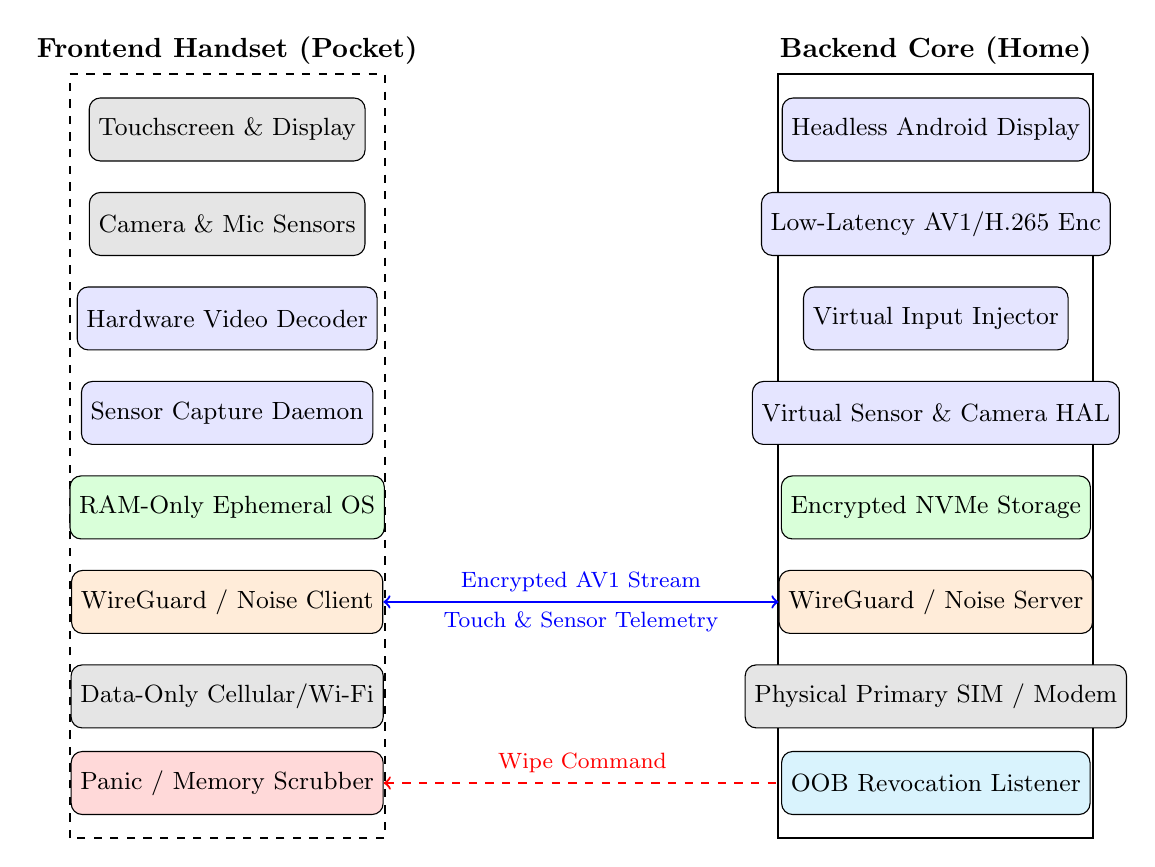
\begin{tikzpicture}[
    box/.style={draw, rectangle, rounded corners, minimum height=0.8cm, text centered, font=\small},
    proc/.style={box, fill=blue!10, minimum width=3.2cm},
    hw/.style={box, fill=gray!20, minimum width=3.2cm},
    sec/.style={box, fill=green!15, minimum width=3.2cm},
    net/.style={box, fill=orange!15, minimum width=2.5cm}
]

    % Frontend Column
    \node[font=\bfseries] at (2,6.5) {Frontend Handset (Pocket)};
    \draw[thick, dashed] (0, -3.5) rectangle (4, 6.2);
    
    \node[hw] (f_screen) at (2, 5.5) {Touchscreen \& Display};
    \node[hw] (f_cam) at (2, 4.3) {Camera \& Mic Sensors};
    \node[proc] (f_decoder) at (2, 3.1) {Hardware Video Decoder};
    \node[proc] (f_capture) at (2, 1.9) {Sensor Capture Daemon};
    \node[sec] (f_ram) at (2, 0.7) {RAM-Only Ephemeral OS};
    \node[net] (f_wg) at (2, -0.5) {WireGuard / Noise Client};
    \node[hw] (f_data_modem) at (2, -1.7) {Data-Only Cellular/Wi-Fi};
    \node[proc, fill=red!15] (f_panic) at (2, -2.8) {Panic / Memory Scrubber};

    % Backend Column
    \node[font=\bfseries] at (11,6.5) {Backend Core (Home)};
    \draw[thick] (9, -3.5) rectangle (13, 6.2);

    \node[proc] (b_render) at (11, 5.5) {Headless Android Display};
    \node[proc] (b_encoder) at (11, 4.3) {Low-Latency AV1/H.265 Enc};
    \node[proc] (b_inject) at (11, 3.1) {Virtual Input Injector};
    \node[proc] (b_vhal) at (11, 1.9) {Virtual Sensor \& Camera HAL};
    \node[sec] (b_storage) at (11, 0.7) {Encrypted NVMe Storage};
    \node[net] (b_wg) at (11, -0.5) {WireGuard / Noise Server};
    \node[hw] (b_sim) at (11, -1.7) {Physical Primary SIM / Modem};
    \node[sec, fill=cyan!15] (b_oob) at (11, -2.8) {OOB Revocation Listener};

    % Network Transits
    \draw[<->, thick, blue] (f_wg) -- node[above, font=\footnotesize] {Encrypted AV1 Stream} node[below, font=\footnotesize] {Touch \& Sensor Telemetry} (b_wg);
    \draw[<-, thick, red, dashed] (f_panic) -- node[above, font=\footnotesize] {Wipe Command} (b_oob);

\end{tikzpicture}
\caption{Detailed architectural blueprint of the Virtual Private Phone framework.}
\label{fig:vpp_detailed_architecture}
\end{figure}

\subsection{The Frontend Node: Ephemeral Thin-Client}
The frontend handset is intentionally designed with an attack surface characterized by minimal state retention:
\begin{itemize}
    \item \textbf{Immutable Root Filesystem ($\texttt{dm-verity}$):} The base operating system is stored in a cryptographically signed, read-only flash partition verified at boot via hardware root of trust. Any unauthorized modification to system binaries causes immediate boot failure.
    \item \textbf{RAM-Disk Volatile Execution ($\texttt{tmpfs}$):} All writable mount points ($\texttt{/tmp}$, $\texttt{/var/run}$, user runtime directories) reside exclusively in volatile dynamic RAM. No persistent user partitions ($\texttt{/data}$) exist on the physical flash memory.
    \item \textbf{Zero Swap / Zero Hibernate:} Virtual memory paging to disk ($\texttt{swap}$) is completely disabled at the kernel level. This prevents page cache remanence and ensures that decrypted video frames or buffers can never be written to non-volatile flash storage.
    \item \textbf{Volatile Display Pipeline:} Decoded video frames from the remote backend are rendered directly to the hardware display controller via zero-copy DMA buffers ($\texttt{dma-buf}$). Frames exist in memory only for the duration of a single refresh cycle ($1/60\text{s}$ or $1/120\text{s}$) before being overwritten by subsequent framebuffers.
\end{itemize}

\subsection{The Backend Node: Persistent Home Core}
The backend core serves as the computational anchor and root of identity:
\begin{itemize}
    \item \textbf{Hardware Execution Environment:} Hosted on physical hardware stationed in the operator's domestic sanctuary. This can take the form of a dedicated, stationary smartphone chassis, a secure embedded system (e.g., ARM64 board with hardware SIM slot), or a hardware-accelerated containerized mobile runtime (e.g., hardened Waydroid instance with GPU passthrough).
    \item \textbf{Hardware Security Module (HSM):} Hardware-backed cryptographic key generation and storage (e.g., Titan M2 or TPM 2.0). All private keys, persistent master keys, and pairing certificates are anchored to the physical silicon of the backend.
    \item \textbf{Primary Telephony and SIM Termination:} The user's primary cellular subscriber identity (pSIM or primary carrier eSIM profile) is physically inserted and terminated on the backend core. Incoming voice calls, SMS messages (including critical 2FA codes), and cellular operator registrations never leave the domestic perimeter.
\end{itemize}

\subsection{The Virtual Hardware Abstraction Layer (V-HAL)}
To achieve full feature parity with an ordinary smartphone, the VPP introduces the Virtual Hardware Abstraction Layer (V-HAL). Traditional remote desktop protocols (e.g., RDP, VNC) only support generic pointer clicks and keystrokes. In contrast, modern mobile operating systems require continuous, rich sensor telemetry:

\subsubsection{1. Multi-Touch and Input Virtualization}
Capacitive touch events on the frontend are captured at 120\,Hz via the kernel's $\texttt{evdev}$ input subsystem. Touch packets include multi-finger tracking IDs, pressure values ($P$), contact area dimensions ($W \times H$), and precise microsecond timestamps:
\begin{equation}
    E_{touch} = \langle id, x, y, p, t_{event} \rangle
\end{equation}
These events are serialized into high-priority UDP datagrams, transmitted over the WireGuard tunnel, and injected into the backend's Android $\texttt{InputManager}$ via a synthetic kernel virtual device ($\texttt{uinput}$). This preserves native gesture recognition, multi-finger pinching, flick scrolling, and edge-swiping.

\subsubsection{2. Ultra-Low Latency Video Streaming Pipeline}
The backend generates display output within a virtual headless display buffer ($1080 \times 2400$ @ 60/120\,fps). Video frames are captured using zero-copy GPU memory access and compressed in real time using hardware-accelerated AV1 or H.265 (HEVC) encoders with ultra-low latency configurations:
\begin{itemize}
    \item \textbf{Zero B-Frames:} Strict I-P-P frame sequences eliminate backward reference buffering delays.
    \item \textbf{Intra-Refresh Cycling:} Instead of periodic, bandwidth-heavy Intra (I) keyframes, the encoder continuously refreshes a rolling vertical slice of macroblocks across successive P-frames, mitigating buffer spikes and packet loss stutter.
    \item \textbf{Adaptive Dynamic Bitrate (ABR):} Bitrate and quantization parameters scale dynamically between 2\,Mbps (constrained LTE) and 25\,Mbps (5G/Wi-Fi) based on real-time network congestion feedback (RFC 8888 RTP congestion control).
\end{itemize}

\subsubsection{3. Bi-Directional Peripheral Virtualization}
\begin{itemize}
    \item \textbf{Camera Bridging:} When the user launches a camera-reliant application on the backend (e.g., document scanner, secure messenger), the backend camera HAL requests a video stream. The frontend activates its physical camera sensor, compresses the video stream locally, and transmits it upstream to the backend's virtual camera driver ($\texttt{v4l2loopback}$), which presents it to the Android runtime as a native hardware sensor.
    \item \textbf{Audio and Microphone Duplexing:} Bi-directional Opus audio channels stream at 48\,kHz with 10\,ms packetization intervals. The frontend microphone stream is piped to the backend's virtual ALSA input, enabling voice calling, voice notes, and audio recording.
    \item \textbf{Sensor and Location Relay:} The frontend's accelerometer, gyroscope, magnetometer, and ambient light sensors are sampled and forwarded upstream. For geolocation, the operator can toggle between forwarding the frontend's physical GPS coordinates (for local navigation) or enforcing the backend's static home location (for absolute operational privacy).
\end{itemize}
